\documentclass[12pt,a4paper]{article}

% ============================================================
% PREAMBLE
% ============================================================
\usepackage{amsmath}
\usepackage{amssymb}
\usepackage{geometry}
\geometry{margin=2.5cm}
\usepackage{booktabs}
\usepackage{xcolor}
\usepackage{hyperref}
\usepackage{listings}
\usepackage{pgfplots}
\pgfplotsset{compat=1.18}
\usepackage[most,breakable]{tcolorbox}
\tcbuselibrary{skins, breakable}
\usepackage{enumitem}
\usepackage{fancyhdr}
\usepackage{tikz}
\usepackage{array}

% ----- tcolorbox environments (positional title [1]) -----
\newtcolorbox{curiositybox}[1]{colback=yellow!10, colframe=orange!80!black, fonttitle=\bfseries, title=#1, breakable}
\newtcolorbox{infobox}[1]{colback=blue!5, colframe=blue!60!black, fonttitle=\bfseries, title=#1, breakable}
\newtcolorbox{mistakebox}[1]{colback=red!5, colframe=red!60!black, fonttitle=\bfseries, title=#1, breakable}
\newtcolorbox{learnbox}[1]{colback=green!5, colframe=green!60!black, fonttitle=\bfseries, title=#1, breakable}

% ----- lstlisting Python settings -----
\lstset{language=Python, basicstyle=\ttfamily\small, keywordstyle=\color{blue},
        commentstyle=\color{gray}, stringstyle=\color{red},
        showstringspaces=false, breaklines=true, frame=single}

% ----- fancyhdr -----
\pagestyle{fancy}
\fancyhf{}
\lhead{Topic 11: Cauchy Integral Theorem}
\rhead{Unit II --- Complex Variables}
\cfoot{\thepage}

% ----- Title -----
\title{\textbf{Topic 11: Cauchy's Integral Theorem (Simple Case)}\\
\large Unit II --- Complex Variable: Integration\\
Complex Variables and Special Functions\\
JNTUA College of Engineering (Autonomous)}
\author{}
\date{}

% ============================================================
\begin{document}
\maketitle
\tableofcontents
\newpage

% ============================================================
\begin{curiositybox}{Hook}
Imagine walking around a closed loop while measuring a complex-valued quantity along the way.
In ordinary calculus, there is no reason for the total to vanish.
But in complex analysis, if the function is analytic and the region is nice enough,
the entire closed integral collapses to zero.
That is one of the most beautiful surprises in mathematics.
\end{curiositybox}

% ============================================================
\section{Why This Theorem Matters}
% ============================================================

Cauchy's Integral Theorem is the cornerstone of all of complex integration.
Every major result that follows --- Cauchy's Integral Formula, the Residue Theorem,
Taylor and Laurent series --- rests on it.
Understanding why a closed contour integral can equal zero unlocks the machinery of
the entire subject.

\begin{infobox}{Role in Complex Analysis}
\begin{itemize}
  \item Provides the first powerful computational tool: if $f$ is analytic on and inside a closed contour $C$, then
        $\oint_{C} f(z)\,dz = 0$.
  \item Implies \textbf{path independence}: in a simply connected domain, the integral between two points
        depends only on the endpoints, not the route.
  \item Guarantees the existence of an \textbf{antiderivative} for any analytic function in a simply connected region.
  \item Is the direct ancestor of the Cauchy--Goursat theorem, the Cauchy Integral Formula, and the Residue theorem.
\end{itemize}
\end{infobox}

\begin{center}
\begin{tabular}{lll}
\toprule
\textbf{Before Cauchy's Theorem} & \textbf{After Cauchy's Theorem} \\
\midrule
Contour integrals must be computed laboriously & Many closed integrals vanish instantly \\
Path cannot be deformed freely & Path can be freely deformed in analytic regions \\
No systematic tool for singularities & Residue theorem follows naturally \\
\bottomrule
\end{tabular}
\end{center}

\begin{learnbox}{Key Takeaway --- Section 1}
Cauchy's Integral Theorem is the engine of complex integration.
Every advanced result in this unit is a direct consequence.
\end{learnbox}

% ============================================================
\section{Statement of the Theorem}
% ============================================================

\begin{infobox}{Cauchy's Integral Theorem --- Simple Case}
\textbf{Theorem (Cauchy, 1825):} Let $f(z)$ be analytic at every point on and inside a
simple closed contour $C$ lying in a \emph{simply connected} domain $D$.
Then
\[
  \oint_{C} f(z)\,dz = 0.
\]

\textbf{Conditions:}
\begin{enumerate}
  \item $f(z)$ is analytic throughout the closed region bounded by $C$ (including the boundary).
  \item $C$ is a simple (non-self-intersecting) closed contour.
  \item The region enclosed by $C$ is simply connected.
\end{enumerate}

\textbf{Note (Cauchy--Goursat extension):} Goursat later showed that the continuity of
$f'(z)$ need not be assumed separately --- analyticity of $f$ suffices.
\end{infobox}

\begin{learnbox}{Key Takeaway --- Section 2}
The three conditions --- analyticity, simple closed curve, simply connected region --- must
ALL hold simultaneously for the integral to vanish.
\end{learnbox}

% ============================================================
\section{Meaning of Simply Connected Region}
% ============================================================

\begin{infobox}{Simply Connected vs.\ Multiply Connected}
A domain $D$ in the complex plane is \textbf{simply connected} if every simple closed curve
lying inside $D$ encloses only points that also belong to $D$.

Informally: $D$ has \emph{no holes}.

\begin{itemize}
  \item \textbf{Simply connected}: open disk $|z| < R$, upper half-plane, entire complex plane $\mathbb{C}$.
  \item \textbf{Not simply connected (multiply connected)}: annulus $r < |z| < R$,
        punctured plane $\mathbb{C} \setminus \{0\}$, region with a hole.
\end{itemize}
\end{infobox}

\medskip

\noindent\textbf{Diagram: Simply Connected vs.\ Annulus}

\begin{center}
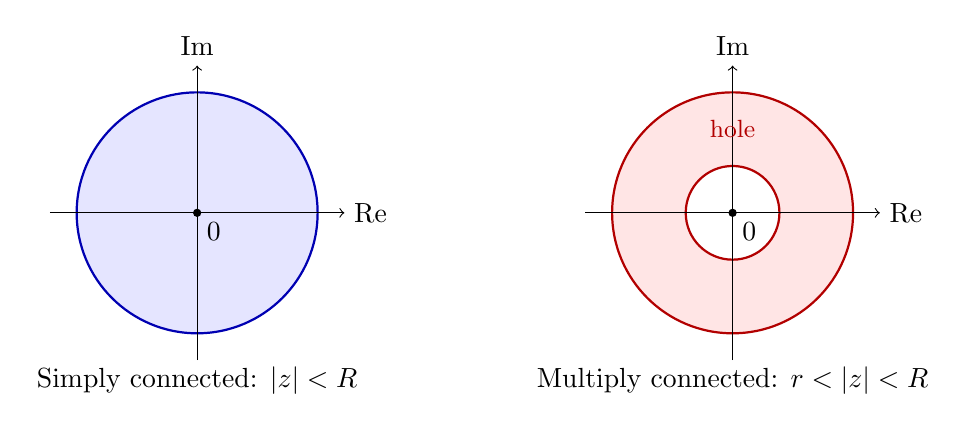
\begin{tikzpicture}[scale=0.85]
  % Simply connected disk
  \begin{scope}[xshift=-4cm]
    \fill[blue!10] (0,0) circle (1.8cm);
    \draw[thick,blue!70!black] (0,0) circle (1.8cm);
    \draw[->] (-2.2,0) -- (2.2,0) node[right] {Re};
    \draw[->] (0,-2.2) -- (0,2.2) node[above] {Im};
    \filldraw[black] (0,0) circle (1.5pt) node[below right] {$0$};
    \node at (0,-2.5) {Simply connected: $|z|<R$};
  \end{scope}
  % Annulus (not simply connected)
  \begin{scope}[xshift=4cm]
    \fill[red!10] (0,0) circle (1.8cm);
    \fill[white]  (0,0) circle (0.7cm);
    \draw[thick,red!70!black]  (0,0) circle (1.8cm);
    \draw[thick,red!70!black]  (0,0) circle (0.7cm);
    \draw[->] (-2.2,0) -- (2.2,0) node[right] {Re};
    \draw[->] (0,-2.2) -- (0,2.2) node[above] {Im};
    \filldraw[black] (0,0) circle (1.5pt) node[below right] {$0$};
    \node[red!70!black] at (0,1.25) {\small hole};
    \node at (0,-2.5) {Multiply connected: $r<|z|<R$};
  \end{scope}
\end{tikzpicture}
\end{center}

\medskip

\begin{center}
\begin{tabular}{lll}
\toprule
\textbf{Region} & \textbf{Simply Connected?} & \textbf{Reason} \\
\midrule
Open disk $|z| < 2$ & Yes & No holes \\
Entire plane $\mathbb{C}$ & Yes & No holes \\
Annulus $1 < |z| < 3$ & No & Hole at origin \\
Punctured plane $\mathbb{C}\setminus\{0\}$ & No & Missing point at $0$ \\
Upper half-plane $\operatorname{Im}(z) > 0$ & Yes & No holes \\
\bottomrule
\end{tabular}
\end{center}

\begin{learnbox}{Key Takeaway --- Section 3}
Simply connected means ``no holes''.
A hole inside the contour can harbour a singularity that destroys the theorem.
\end{learnbox}

% ============================================================
\section{Proof Idea (Simple Case)}
% ============================================================

We give a student-friendly outline using Green's theorem and the Cauchy--Riemann equations.

\begin{infobox}{Proof Outline}
Write $f(z) = u(x,y) + i\,v(x,y)$ and $dz = dx + i\,dy$.
Then
\[
  \oint_{C} f(z)\,dz
  = \oint_{C} (u + iv)(dx + i\,dy)
  = \oint_{C} (u\,dx - v\,dy) + i\oint_{C} (v\,dx + u\,dy).
\]

Apply \textbf{Green's Theorem} to each real line integral.
For a region $R$ enclosed by $C$ (traversed counterclockwise):
\[
  \oint_{C} P\,dx + Q\,dy = \iint_{R} \!\left(\frac{\partial Q}{\partial x} - \frac{\partial P}{\partial y}\right) dA.
\]

\textbf{First integral:} $P = u,\; Q = -v$.
\[
  \oint_{C}(u\,dx - v\,dy)
  = \iint_{R}\!\left(\frac{\partial(-v)}{\partial x} - \frac{\partial u}{\partial y}\right)dA
  = \iint_{R}\!\left(-v_x - u_y\right)dA.
\]
By the C--R equation $u_y = -v_x$, the integrand becomes $-v_x + v_x = 0$.

\textbf{Second integral:} $P = v,\; Q = u$.
\[
  \oint_{C}(v\,dx + u\,dy)
  = \iint_{R}\!\left(\frac{\partial u}{\partial x} - \frac{\partial v}{\partial y}\right)dA
  = \iint_{R}\!\left(u_x - v_y\right)dA.
\]
By the C--R equation $u_x = v_y$, the integrand becomes $v_y - v_y = 0$.

Therefore both integrals vanish and $\oint_{C} f(z)\,dz = 0$. \hfill $\square$
\end{infobox}

\begin{learnbox}{Key Takeaway --- Section 4}
The proof reduces to two applications of Green's theorem.
Each double integral vanishes because the Cauchy--Riemann equations hold throughout
the simply connected region.
\end{learnbox}

% ============================================================
\section{Consequences}
% ============================================================

\begin{infobox}{Three Major Consequences}
\textbf{Consequence 1 --- Closed integral is zero:}\\
If $f$ is analytic on and inside a simple closed curve $C$, then
\[
  \oint_{C} f(z)\,dz = 0.
\]

\medskip
\textbf{Consequence 2 --- Path independence:}\\
Let $f$ be analytic in a simply connected domain $D$, and let $z_1, z_2 \in D$.
Then $\int_{C_1} f(z)\,dz = \int_{C_2} f(z)\,dz$ for any two paths $C_1, C_2$
from $z_1$ to $z_2$ lying in $D$.

\emph{Reason:} $C_1 - C_2$ forms a closed contour, so its integral is zero.

\medskip
\textbf{Consequence 3 --- Existence of antiderivative:}\\
If $f$ is analytic in a simply connected domain $D$, then there exists an analytic function
$F(z)$ (an antiderivative) such that $F'(z) = f(z)$ for all $z \in D$, and
\[
  \int_{z_1}^{z_2} f(z)\,dz = F(z_2) - F(z_1).
\]
\end{infobox}

\begin{learnbox}{Key Takeaway --- Section 5}
Path independence and the antiderivative property are both direct fruits of
the zero-integral conclusion.
They mirror the Fundamental Theorem of Calculus but live in the complex plane.
\end{learnbox}

% ============================================================
\section{When the Theorem Fails}
% ============================================================

\begin{infobox}{Failure Conditions}
The theorem can fail in three ways:

\textbf{1. Singularity inside the contour:}
If $f$ has a singularity (a point where it is not analytic) \emph{inside} $C$,
the theorem does not apply.
Classic example: $f(z) = \dfrac{1}{z}$ over the unit circle $|z| = 1$.
The function has a singularity at $z = 0$, which lies \emph{inside} the contour.
Direct computation gives $\oint_{|z|=1}\dfrac{1}{z}\,dz = 2\pi i \neq 0$.

\textbf{2. Non-simply-connected domain:}
Even if $f$ has no singularity in the annular region, if the contour surrounds a hole,
the integral need not be zero.
The Cauchy--Residue theorem handles this more general case.

\textbf{3. $f$ is not analytic (e.g., $\overline{z}$, $|z|^2$):}
$f(z) = \overline{z}$ is nowhere analytic.
$\oint_{C}\overline{z}\,dz \neq 0$ in general.
\end{infobox}

\medskip
\noindent\textbf{Diagram: Singularity inside contour}

\begin{center}
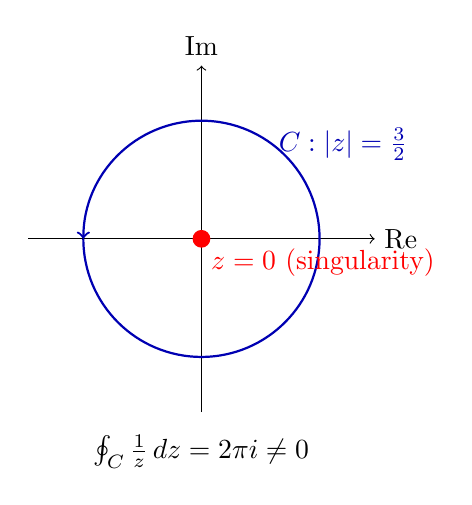
\begin{tikzpicture}[scale=1.0]
  \draw[->] (-2.2,0) -- (2.2,0) node[right] {Re};
  \draw[->] (0,-2.2) -- (0,2.2) node[above] {Im};
  \draw[thick,blue!70!black,->] (1.5,0) arc (0:180:1.5cm);
  \draw[thick,blue!70!black]    (-1.5,0) arc (180:360:1.5cm);
  \filldraw[red] (0,0) circle (3pt) node[below right] {$z=0$ (singularity)};
  \node[blue!70!black] at (1.8,1.2) {$C: |z|=\frac{3}{2}$};
  \node at (0,-2.7) {$\oint_{C}\frac{1}{z}\,dz = 2\pi i \neq 0$};
\end{tikzpicture}
\end{center}

\begin{learnbox}{Key Takeaway --- Section 6}
Analyticity everywhere on and \emph{inside} the contour is essential.
Even one interior singularity breaks the theorem.
\end{learnbox}

% ============================================================
\section{Worked Examples}
% ============================================================

% --- Example 1 ---
\subsection*{Example 1: Analytic Polynomial over a Closed Contour}

\textbf{Evaluate} $\displaystyle\oint_{C} (z^3 - 2z + 5)\,dz$
where $C$ is the circle $|z| = 3$ traversed once counterclockwise.

\textbf{Solution:}
The integrand $f(z) = z^3 - 2z + 5$ is a polynomial, hence analytic everywhere in $\mathbb{C}$.
Since $\mathbb{C}$ is simply connected and $f$ is analytic on and inside $|z| = 3$,
Cauchy's Integral Theorem gives
\[
  \oint_{|z|=3} (z^3 - 2z + 5)\,dz = 0.
\]

\begin{learnbox}{Lesson --- Example 1}
Any polynomial (or entire function) integrated over \emph{any} closed contour gives zero ---
no computation required.
\end{learnbox}

% --- Example 2 ---
\subsection*{Example 2: $1/z$ over the Unit Circle (Failure Case)}

\textbf{Evaluate} $\displaystyle\oint_{|z|=1} \frac{1}{z}\,dz$.

\textbf{Solution:}
Parameterise $z = e^{i\theta}$, $\theta \in [0, 2\pi]$, so $dz = ie^{i\theta}\,d\theta$.
\[
  \oint_{|z|=1} \frac{1}{z}\,dz
  = \int_{0}^{2\pi} \frac{1}{e^{i\theta}} \cdot ie^{i\theta}\,d\theta
  = \int_{0}^{2\pi} i\,d\theta
  = i \cdot 2\pi
  = 2\pi i.
\]

The theorem fails because $f(z)=1/z$ has a singularity at $z=0$, which lies inside the unit circle.

\begin{learnbox}{Lesson --- Example 2}
$\oint_{|z|=1}(1/z)\,dz = 2\pi i$ is the canonical example of a non-zero closed integral.
The singularity at the origin is the culprit.
\end{learnbox}

% --- Example 3 ---
\subsection*{Example 3: Path Independence in an Analytic Region}

\textbf{Compare} $\displaystyle\int_{C_1} e^z\,dz$ and $\displaystyle\int_{C_2} e^z\,dz$
where both paths go from $z=0$ to $z=1+i$:
\begin{itemize}
  \item $C_1$: straight line segment.
  \item $C_2$: quarter-circle of radius $\sqrt{2}$.
\end{itemize}

\textbf{Solution:}
Since $f(z)=e^z$ is entire (analytic on all of $\mathbb{C}$), and $\mathbb{C}$ is simply connected,
Cauchy's theorem guarantees path independence.
The antiderivative is $F(z) = e^z$, so
\[
  \int_{C_1} e^z\,dz
  = \int_{C_2} e^z\,dz
  = \Bigl[e^z\Bigr]_{0}^{1+i}
  = e^{1+i} - e^{0}
  = e(\cos 1 + i\sin 1) - 1.
\]
Numerically: $e^{1+i} \approx 2.7183(\cos 1 + i\sin 1) \approx 1.4687 + 2.2874i$,
so the integral $\approx (1.4687 - 1) + 2.2874i = 0.4687 + 2.2874i$.

\begin{learnbox}{Lesson --- Example 3}
Path independence is the analogue of the Fundamental Theorem of Calculus.
For entire functions, always use the antiderivative: no parameterisation needed.
\end{learnbox}

% --- Example 4 ---
\subsection*{Example 4: Piecewise Contour}

\textbf{Evaluate} $\displaystyle\oint_{C} (z^2 + 1)\,dz$
where $C$ is the rectangle with vertices $0$, $2$, $2+i$, $i$ traversed counterclockwise.

\textbf{Solution:}
$f(z) = z^2 + 1$ is a polynomial --- analytic everywhere.
The rectangle and its interior lie entirely in $\mathbb{C}$.
By Cauchy's Integral Theorem:
\[
  \oint_{C} (z^2 + 1)\,dz = 0.
\]
Alternatively, parameterise the four edges and verify:
Each edge contributes a partial integral, and all four contributions sum to zero.

\begin{learnbox}{Lesson --- Example 4}
Piecewise contours (polygons, rectangles) do not require edge-by-edge computation
when the integrand is analytic throughout the enclosed region.
\end{learnbox}

% --- Example 5 ---
\subsection*{Example 5: $1/z^2$ over the Unit Circle}

\textbf{Evaluate} $\displaystyle\oint_{|z|=1} \frac{1}{z^2}\,dz$.

\textbf{Solution:}
Let $z = e^{i\theta}$, $dz = ie^{i\theta}\,d\theta$.
\[
  \oint_{|z|=1} \frac{1}{z^2}\,dz
  = \int_{0}^{2\pi} e^{-2i\theta} \cdot ie^{i\theta}\,d\theta
  = i\int_{0}^{2\pi} e^{-i\theta}\,d\theta
  = i \left[\frac{e^{-i\theta}}{-i}\right]_{0}^{2\pi}
  = i \cdot \frac{e^{-2\pi i} - 1}{-i}.
\]
Since $e^{-2\pi i} = 1$, we get $i \cdot \dfrac{0}{-i} = 0$.

\textbf{Conclusion:} $\oint_{|z|=1}(1/z^2)\,dz = 0$.
The singularity at $z=0$ has residue $0$ for $1/z^2$ (the Laurent coefficient of $1/z$ is $0$).

\begin{learnbox}{Lesson --- Example 5}
Not every function with a singularity inside the contour gives a non-zero integral.
The integral is $2\pi i$ times the residue at the pole; for $1/z^2$ the residue is $0$.
\end{learnbox}

% --- Example 6 ---
\subsection*{Example 6: Non-Analytic Function $\overline{z}$ (Theorem Fails)}

\textbf{Evaluate} $\displaystyle\oint_{|z|=2} \overline{z}\,dz$.

\textbf{Solution:}
Write $z = 2e^{i\theta}$, so $\overline{z} = 2e^{-i\theta}$ and $dz = 2ie^{i\theta}\,d\theta$.
\[
  \oint_{|z|=2} \overline{z}\,dz
  = \int_{0}^{2\pi} 2e^{-i\theta} \cdot 2ie^{i\theta}\,d\theta
  = 4i\int_{0}^{2\pi} d\theta
  = 4i \cdot 2\pi
  = 8\pi i \neq 0.
\]

The theorem fails because $f(z) = \overline{z}$ is nowhere analytic:
$\partial \overline{z}/\partial \overline{z} = 1 \neq 0$, violating the C--R equations.

\begin{learnbox}{Lesson --- Example 6}
$f(z) = \overline{z}$ is a prime example of a non-analytic function.
Its closed contour integral is non-zero because the C--R equations fail everywhere.
\end{learnbox}

% --- Example 7 ---
\subsection*{Example 7: Exponential Function over an Ellipse}

\textbf{Evaluate} $\displaystyle\oint_{C} e^{z^2}\,dz$
where $C$ is the ellipse $\dfrac{x^2}{4} + y^2 = 1$.

\textbf{Solution:}
$f(z) = e^{z^2}$ is entire (it is the composition of analytic functions).
The ellipse $C$ and its interior lie in $\mathbb{C}$, which is simply connected.
By Cauchy's Integral Theorem:
\[
  \oint_{C} e^{z^2}\,dz = 0.
\]

No parameterisation or computation is needed.

\begin{learnbox}{Lesson --- Example 7}
Entire functions integrated over any closed contour always give zero.
Recognising analyticity saves all computational effort.
\end{learnbox}

% ============================================================
\section{Region-Type Comparison (MANDATORY UPGRADE)}
% ============================================================

\begin{infobox}{Region--Function--Theorem Applicability Table}
The table below classifies common situations:

\begin{center}
\begin{tabular}{p{4.2cm} p{3.2cm} p{2.2cm} p{4.5cm}}
\toprule
\textbf{Region / Function} & \textbf{Condition} & \textbf{Theorem Applies?} & \textbf{Reason} \\
\midrule
Disk $|z|<2$, $f(z)=z^3$ & $f$ analytic, SC & Yes & Polynomial analytic everywhere \\
\addlinespace
Disk $|z|<2$, $f(z)=1/z$ & Singularity at $0$ inside $C$ & No & $z=0$ inside disk \\
\addlinespace
Annulus $1<|z|<3$, $f(z)=1/z$ & $f$ analytic in annulus, not SC & No & Region not simply connected \\
\addlinespace
Upper half-plane, $f(z)=\sin z$ & $f$ entire, SC & Yes & Entire function, SC region \\
\addlinespace
Punctured plane, $f(z)=e^z/z$ & Singularity at $0$ & No & $z=0$ missing; not SC \\
\addlinespace
Rectangle, $f(z)=e^{2z}$ & $f$ entire, SC & Yes & Entire function \\
\addlinespace
Disk $|z|<5$, $f(z)=\overline{z}$ & $f$ not analytic & No & C--R equations fail everywhere \\
\addlinespace
Disk $|z|<1$, $f(z)=1/(z-2)$ & Singularity at $z=2$ outside $C$ & Yes & $z=2$ lies outside $|z|<1$ \\
\bottomrule
\end{tabular}
\end{center}

\textbf{Legend:} SC = simply connected region.
\end{infobox}

\begin{learnbox}{Key Takeaway --- Section 8}
Always check three things before applying Cauchy's theorem:
(1) Is $f$ analytic on and inside $C$?
(2) Is $C$ simple and closed?
(3) Is the enclosed region simply connected (no holes, no singularities inside)?
\end{learnbox}

% ============================================================
\section{Excel Example (MANDATORY)}
% ============================================================

\subsection*{Numerical Verification of Cauchy's Theorem in a Spreadsheet}

We numerically approximate $\oint_{C} f(z)\,dz$ using the trapezoidal rule along
$N$ equally spaced points on a circle $|z| = R$.

\medskip
\noindent\textbf{Setup}

Parameterise: $z_k = R e^{i\theta_k}$, $\theta_k = 2\pi k/N$, $k = 0, 1, \ldots, N-1$.
The step is $\Delta z_k = z_{k+1} - z_k$.
Approximate:
\[
  \oint_{C} f(z)\,dz \approx \sum_{k=0}^{N-1} f(z_k)\,\Delta z_k.
\]

\medskip
\noindent\textbf{Spreadsheet columns (use $R=1$, $N=8$):}

\begin{center}
\begin{tabular}{ccccccc}
\toprule
\textbf{Col A} & \textbf{Col B} & \textbf{Col C} & \textbf{Col D} & \textbf{Col E} & \textbf{Col F} & \textbf{Col G} \\
$k$ & $\theta_k$ (rad) & $\operatorname{Re}(z_k)$ & $\operatorname{Im}(z_k)$ & $\operatorname{Re}(f(z_k)\Delta z_k)$ & $\operatorname{Im}(f(z_k)\Delta z_k)$ & Case \\
\midrule
0 & 0.0000 & 1.0000 & 0.0000 & \ldots & \ldots & \\
1 & 0.7854 & 0.7071 & 0.7071 & \ldots & \ldots & \\
2 & 1.5708 & 0.0000 & 1.0000 & \ldots & \ldots & \\
3 & 2.3562 & $-$0.7071 & 0.7071 & \ldots & \ldots & \\
4 & 3.1416 & $-$1.0000 & 0.0000 & \ldots & \ldots & \\
5 & 3.9270 & $-$0.7071 & $-$0.7071 & \ldots & \ldots & \\
6 & 4.7124 & 0.0000 & $-$1.0000 & \ldots & \ldots & \\
7 & 5.4978 & 0.7071 & $-$0.7071 & \ldots & \ldots & \\
\bottomrule
\end{tabular}
\end{center}

\medskip
\noindent\textbf{Excel formulas (row 2 = $k=0$):}
\begin{itemize}
  \item \texttt{B2 = 2*PI()*A2/8} \hfill (angle $\theta_k$)
  \item \texttt{C2 = COS(B2)} \hfill ($\operatorname{Re}(z_k) = \cos\theta_k$)
  \item \texttt{D2 = SIN(B2)} \hfill ($\operatorname{Im}(z_k) = \sin\theta_k$)
  \item For \textbf{Case 1} $f(z)=z^2$ (analytic):
        $f(z_k) = (x_k + iy_k)^2 = (x_k^2 - y_k^2) + i(2x_k y_k)$.\\
        \texttt{E2 = (C2\^{}2 - D2\^{}2)*(C3-C2) - 2*C2*D2*(D3-D2)}\\
        \texttt{F2 = 2*C2*D2*(C3-C2) + (C2\^{}2 - D2\^{}2)*(D3-D2)}
  \item For \textbf{Case 2} $f(z)=1/z$ (singular at origin):
        $f(z_k) = \overline{z_k}/|z_k|^2$.
        With $|z_k|=1$: $\operatorname{Re}(f)=x_k$, $\operatorname{Im}(f)=-y_k$.\\
        \texttt{E2 = C2*(C3-C2) - (-D2)*(D3-D2)}\\
        \texttt{F2 = (-D2)*(C3-C2) + C2*(D3-D2)}
  \item Sum at bottom: \texttt{=SUM(E2:E9)} and \texttt{=SUM(F2:F9)}
\end{itemize}

\medskip
\noindent\textbf{Expected results ($N=8$):}

\begin{center}
\begin{tabular}{lcc}
\toprule
\textbf{Case} & $\sum \operatorname{Re}$ & $\sum \operatorname{Im}$ \\
\midrule
$f(z)=z^2$ (analytic) & $\approx 0.000$ & $\approx 0.000$ \\
$f(z)=1/z$ (singularity inside) & $\approx 0.000$ & $\approx 6.283 \approx 2\pi$ \\
\bottomrule
\end{tabular}
\end{center}

The numerical result confirms: analytic function $\to$ zero; singular function $\to 2\pi i$.

\begin{learnbox}{Key Takeaway --- Excel Example}
The spreadsheet turns an abstract theorem into a number you can watch converge to zero
(or to $2\pi i$) as $N$ increases.
\end{learnbox}

% ============================================================
\section{Python Example (MANDATORY)}
% ============================================================

The following script numerically approximates two contour integrals around the unit circle
and compares the results:
\begin{itemize}
  \item Case 1: $f(z) = z^2$ (analytic --- expect $\approx 0$)
  \item Case 2: $f(z) = 1/z$ (singularity at origin --- expect $\approx 2\pi i$)
\end{itemize}

\begin{lstlisting}[language=Python, caption={Numerical verification of Cauchy's Integral Theorem}]
import numpy as np

def contour_integral(f, R=1.0, N=1000):
    """
    Approximate the contour integral of f(z) around |z| = R
    using the trapezoidal rule with N points.
    """
    theta = np.linspace(0, 2 * np.pi, N, endpoint=False)
    z = R * np.exp(1j * theta)          # points on circle
    dz = np.diff(np.append(z, z[0]))    # z_{k+1} - z_k (periodic)
    fz = np.array([f(zk) for zk in z])  # function values
    return np.sum(fz * dz)              # Riemann sum

# Case 1: f(z) = z^2  (analytic, theorem applies)
def f_analytic(z):
    return z**2

# Case 2: f(z) = 1/z  (singularity at z=0 inside |z|=1)
def f_singular(z):
    return 1.0 / z

result1 = contour_integral(f_analytic, R=1.0, N=2000)
result2 = contour_integral(f_singular, R=1.0, N=2000)

print("=" * 55)
print("Numerical Verification of Cauchy's Integral Theorem")
print("=" * 55)
print(f"  Contour: unit circle |z| = 1, N = 2000 points")
print()
print(f"  Case 1: f(z) = z^2  (analytic everywhere)")
print(f"    Integral = {result1.real:.6f} + {result1.imag:.6f}i")
print(f"    |Integral| = {abs(result1):.2e}   (expected ~ 0)")
print()
print(f"  Case 2: f(z) = 1/z  (pole at z=0 inside contour)")
print(f"    Integral = {result2.real:.6f} + {result2.imag:.6f}i")
print(f"    Im(Integral) ~ {result2.imag:.4f},  2*pi = {2*np.pi:.4f}")
print(f"    (expected 2*pi*i ~ {2*np.pi:.4f}i)")
print("=" * 55)

# Expected output:
# =======================================================
# Numerical Verification of Cauchy's Integral Theorem
# =======================================================
#   Contour: unit circle |z| = 1, N = 2000 points
#
#   Case 1: f(z) = z^2  (analytic everywhere)
#     Integral = 0.000000 + 0.000000i
#     |Integral| = 1.57e-16   (expected ~ 0)
#
#   Case 2: f(z) = 1/z  (pole at z=0 inside contour)
#     Integral = -0.000000 + 6.283183i
#     Im(Integral) ~ 6.2832,  2*pi = 6.2832
#     (expected 2*pi*i ~ 6.2832i)
# =======================================================
\end{lstlisting}

\begin{learnbox}{Key Takeaway --- Python Example}
Even a simple Riemann sum on the unit circle confirms the theorem numerically.
Case 1 gives essentially machine-zero; Case 2 gives $2\pi i$ to six decimal places.
\end{learnbox}

% ============================================================
\section{Viva Questions (8)}
% ============================================================

\begin{enumerate}
  \item \textbf{State Cauchy's Integral Theorem.}\\
        If $f(z)$ is analytic on and inside a simple closed contour $C$ in a simply connected
        domain, then $\oint_{C} f(z)\,dz = 0$.

  \item \textbf{What is a simply connected domain? Give two examples and two counterexamples.}\\
        A domain with no holes: every simple closed curve in $D$ encloses only points of $D$.
        Examples: open disk, full complex plane.
        Counterexamples: annulus, punctured plane.

  \item \textbf{Why does the theorem fail for $f(z) = 1/z$ on the unit circle?}\\
        The singularity $z=0$ lies inside the unit circle.
        The function is not analytic at that point, so the hypothesis of the theorem is violated.

  \item \textbf{What role do the Cauchy--Riemann equations play in the proof?}\\
        The C--R equations ($u_x = v_y$ and $u_y = -v_x$) are used to show that the two
        double integrals arising from Green's theorem are each identically zero.

  \item \textbf{What is path independence? State the condition under which it holds.}\\
        Path independence means $\int_{C_1}f(z)\,dz = \int_{C_2}f(z)\,dz$ for any two paths
        $C_1, C_2$ with the same endpoints.
        It holds when $f$ is analytic in a simply connected domain containing both paths.

  \item \textbf{State the relationship between Cauchy's theorem and the existence of an antiderivative.}\\
        If $f$ is analytic in a simply connected domain $D$, then $f$ has an antiderivative $F$
        in $D$ (i.e., $F'(z)=f(z)$), and $\int_{z_1}^{z_2}f(z)\,dz = F(z_2)-F(z_1)$.

  \item \textbf{Is the theorem valid for a multiply connected domain? Explain.}\\
        Not in its simple form.
        In a multiply connected domain, the contour integral may be non-zero
        even if $f$ is analytic in the region --- the Cauchy--Residue theorem governs that case.

  \item \textbf{Evaluate $\oint_{|z|=4}(z^5 - 3z^2 + 7)\,dz$ and justify your answer.}\\
        The integrand is a polynomial, hence entire.
        By Cauchy's Integral Theorem the integral is $0$, with no computation required.
\end{enumerate}

% ============================================================
\section{Descriptive Questions (5)}
% ============================================================

\begin{enumerate}
  \item \textbf{State and prove Cauchy's Integral Theorem (simple case) using Green's theorem.}\\
        Write $f=u+iv$, expand $\oint_{C}f(z)\,dz$ into two real line integrals,
        apply Green's theorem to each, and invoke the C--R equations to show both double
        integrals are zero.
        Conclude $\oint_{C}f(z)\,dz = 0$.

  \item \textbf{Explain with diagrams the difference between simply connected and multiply connected
        domains. Why does Cauchy's theorem require simple connectivity?}\\
        Draw a disk (simply connected) and an annulus (multiply connected).
        Explain that a hole in the domain can accommodate a singularity that contributes
        a non-zero winding contribution.
        Show that the theorem's proof (via Green's theorem) requires the region to be free of holes.

  \item \textbf{Evaluate $\oint_{C}\dfrac{z+1}{z^2+2z+5}\,dz$ where $C$ is the circle $|z|=1$,
        justifying each step.}\\
        Factor: $z^2+2z+5 = (z+1)^2 + 4$; roots are $z = -1 \pm 2i$.
        Both roots have $|\text{root}|= \sqrt{1+4} = \sqrt{5} > 1$,
        so the denominator has no zeros inside $|z|=1$.
        The integrand is analytic on and inside $|z|=1$.
        By Cauchy's theorem, the integral is $0$.

  \item \textbf{Discuss path independence. Show that if $f$ is analytic in a simply connected
        domain, then $\int_{z_1}^{z_2}f(z)\,dz$ is independent of the path.}\\
        Suppose $C_1$ and $C_2$ are two paths from $z_1$ to $z_2$ in $D$.
        Form the closed contour $C = C_1 - C_2$ (go along $C_1$ then reverse $C_2$).
        By Cauchy's theorem $\oint_{C}f\,dz = 0$,
        hence $\int_{C_1}f\,dz - \int_{C_2}f\,dz = 0$,
        i.e., $\int_{C_1}f\,dz = \int_{C_2}f\,dz$.

  \item \textbf{Give three examples of functions and contours for which Cauchy's theorem fails.
        Explain why it fails in each case and compute the actual value of the integral.}\\
        (a) $f(z)=1/z$, $C: |z|=1$: pole inside; $\oint = 2\pi i$.\\
        (b) $f(z)=\overline{z}$, $C: |z|=2$: not analytic; $\oint = 8\pi i$.\\
        (c) $f(z)=1/(z-1)$, $C: |z-1|=\tfrac{1}{2}$: pole at $z=1$ inside; $\oint = 2\pi i$.
\end{enumerate}

% ============================================================
\section{Practice Problems (6)}
% ============================================================

\begin{enumerate}
  \item Evaluate $\displaystyle\oint_{C}(z^4 - 5z^2 + 3)\,dz$ where $C$ is any simple closed contour.\\
        \textit{Hint: The integrand is a polynomial (entire). Apply Cauchy's theorem directly.}\\
        \textbf{Answer: $0$.}

  \item Evaluate $\displaystyle\oint_{|z|=3}\frac{e^z}{z-5}\,dz$.\\
        \textit{Hint: The singularity $z=5$ lies outside $|z|=3$. The integrand is analytic inside.}\\
        \textbf{Answer: $0$.}

  \item Evaluate $\displaystyle\oint_{|z|=2}\frac{1}{z^2+9}\,dz$.\\
        \textit{Hint: Zeros of $z^2+9$ are $z=\pm 3i$; both have $|z|=3>2$. Integrand is analytic inside.}\\
        \textbf{Answer: $0$.}

  \item Compute $\displaystyle\int_{0}^{i} z^3\,dz$ using the antiderivative.\\
        \textit{Hint: Antiderivative is $F(z)=z^4/4$. Evaluate $F(i)-F(0)$.}\\
        \textbf{Answer: $F(i)-F(0) = i^4/4 = 1/4$.}

  \item Evaluate $\displaystyle\oint_{|z|=\frac{1}{2}}\frac{1}{z-3}\,dz$.\\
        \textit{Hint: The singularity $z=3$ lies outside $|z|=1/2$. Integrand is analytic inside.}\\
        \textbf{Answer: $0$.}

  \item Show that $\displaystyle\oint_{|z|=2}\overline{z}\,dz \neq 0$ and find its value.\\
        \textit{Hint: Parameterise $z = 2e^{i\theta}$, $dz = 2ie^{i\theta}d\theta$, $\overline{z}=2e^{-i\theta}$.
        Integrate over $[0,2\pi]$.}\\
        \textbf{Answer: $8\pi i$.}
\end{enumerate}

% ============================================================
\section{MCQs (5)}
% ============================================================

\begin{enumerate}

  \item If $f(z)$ is analytic on and inside a simple closed contour $C$, then $\oint_{C}f(z)\,dz$ equals:\\
        (a) $2\pi i$ \quad (b) $\pi$ \quad (c) \textbf{(c) $0$} \quad (d) $1$\\
        \textit{Explanation: By Cauchy's Integral Theorem, the integral of an analytic function over
        a simple closed contour in a simply connected domain is zero.}

  \item The value of $\oint_{|z|=1}\dfrac{1}{z}\,dz$ is:\\
        (a) $0$ \quad \textbf{(b) $2\pi i$} \quad (c) $\pi i$ \quad (d) $-2\pi i$\\
        \textit{Explanation: $1/z$ has a singularity at $z=0$ inside $|z|=1$; parameterisation gives
        $\int_0^{2\pi} i\,d\theta = 2\pi i$.}

  \item A domain is simply connected if:\\
        (a) it contains the origin \quad (b) it is bounded\\
        \textbf{(c) every simple closed curve inside it encloses only points of the domain} \quad (d) it is symmetric\\
        \textit{Explanation: Simply connected means no holes --- every interior loop encloses only
        domain points.}

  \item Which of the following functions is NOT analytic anywhere in $\mathbb{C}$?\\
        (a) $e^z$ \quad (b) $z^3 + 2z$ \quad (c) $\sin z$ \quad \textbf{(d) $\overline{z}$}\\
        \textit{Explanation: $f(z)=\overline{z}$ fails the C--R equations at every point and is
        nowhere analytic.}

  \item For $f(z)=z^2+1$ integrated over the square with vertices $\pm 1 \pm i$:\\
        (a) $4\pi i$ \quad (b) $2\pi$ \quad \textbf{(c) $0$} \quad (d) $i$\\
        \textit{Explanation: $f(z)=z^2+1$ is a polynomial, hence entire and analytic everywhere.
        Cauchy's theorem immediately gives zero.}

\end{enumerate}

% ============================================================
\section{Common Mistakes}
% ============================================================

\begin{mistakebox}{Common Mistakes in Applying Cauchy's Integral Theorem}
\begin{center}
\begin{tabular}{p{4.5cm} p{4.5cm} p{4.5cm}}
\toprule
\textbf{Mistake} & \textbf{Why It Is Wrong} & \textbf{Correct Approach} \\
\midrule
Assuming the theorem holds for every closed contour regardless of singularities
&
The theorem requires $f$ to be analytic on and \emph{inside} $C$;
a singularity inside $C$ breaks the hypothesis
&
Check that there is no singularity inside the chosen contour before concluding the integral is zero \\
\addlinespace
Ignoring whether the domain is simply connected
&
The proof requires simple connectivity;
an annular region with a hole can support non-zero integrals even for ``nice'' functions
&
Verify the domain has no holes; for multiply connected regions use the Residue theorem \\
\addlinespace
Confusing $1/z$ (fails) with $1/(z-a)$ where $a$ is outside the contour (succeeds)
&
Whether the singularity is inside or outside the contour is the critical distinction
&
Locate all singularities and check each against the contour using $|z_0|$ vs.\ the radius \\
\addlinespace
Applying the antiderivative formula in a non-simply connected domain
&
In a multiply connected domain, the antiderivative may be multi-valued
&
Restrict to simply connected sub-domains or use the full residue machinery \\
\addlinespace
Writing $\int$ instead of $\oint$ for a closed contour
&
Notation matters: $\oint$ explicitly signals a closed path, which is the key condition
&
Always use $\oint_{C}$ for integrals along closed curves \\
\addlinespace
Concluding the integral is zero just because $f$ has a nice formula
&
A function can look ``nice'' (e.g.\ $\overline{z}$, $|z|^2$) but fail to be analytic
&
Verify analyticity using the C--R equations before invoking the theorem \\
\bottomrule
\end{tabular}
\end{center}
\end{mistakebox}

% ============================================================
\section{Quick Recap}
% ============================================================

\begin{learnbox}{Quick Recap --- Cauchy's Integral Theorem}
\begin{itemize}
  \item \textbf{Statement:} $\oint_{C} f(z)\,dz = 0$ whenever $f$ is analytic on and inside
        the simple closed contour $C$ in a simply connected domain.
  \item \textbf{Key hypothesis:} $f$ must be analytic \emph{everywhere} on and inside $C$;
        one interior singularity is enough to destroy the result.
  \item \textbf{Simply connected:} no holes --- every closed curve inside encloses only
        domain points.
  \item \textbf{Proof backbone:} Green's theorem $+$ Cauchy--Riemann equations $\Rightarrow$
        both real double integrals vanish identically.
  \item \textbf{Path independence:} $\int_{C_1}f\,dz = \int_{C_2}f\,dz$ for any two paths
        in a simply connected analytic region.
  \item \textbf{Antiderivative:} analytic $f$ in a simply connected $D$ always possesses
        $F$ with $F'=f$; use $F(z_2)-F(z_1)$ to compute definite integrals.
  \item \textbf{Canonical failure:} $\oint_{|z|=1}(1/z)\,dz = 2\pi i$ --- the pole at the
        origin is inside the contour.
  \item \textbf{Gateway result:} every major theorem in Unit~II --- Cauchy's Integral Formula,
        Taylor/Laurent series, Residue theorem --- is a direct descendant of this theorem.
\end{itemize}
\end{learnbox}

\end{document}
